% GAME_HARD_01_PRESENTATION_INTRODUCTION.tex
\section{Introduction}

% GRAPHICS VERIFICATION
% Developed Tile-Based Deferred Shading as part of project.
% Quick description of what Tile-Based Deferred Shading is and what it's for.
% Completed development on my system.
% Cried out in joy to my collegues, having completed a major milestone.
% Pushed to Git repository, the others enthuastically pulling.
% Not functioning on the others' systems.
% Turned out I was the only one with an AMD video card, the others all having NVIDIA.
% Issue, visualized in images below, was caused by the AMD drivers being somewhat nicer in terms of synchronization issues.
% (Note that the attached images aren't actually images of the problem, but picture somewhat what it looked like on NVIDIA systems. The images actually portray the effects of overriding the block-wise limit of pointlights inherent in the Tile-Based Deferred Shading solution).
% Problem may have been detected if I'd used a reference driver for verification, to rid dependency to third-party drivers and hardware.
\subsection{Graphics Verification}
\begin{frame}
\frametitle{GRAPHICS VERIFICATION}

\begin{figure}[ht]
  \begin{minipage}[b]{0.3\linewidth}
    \centering
    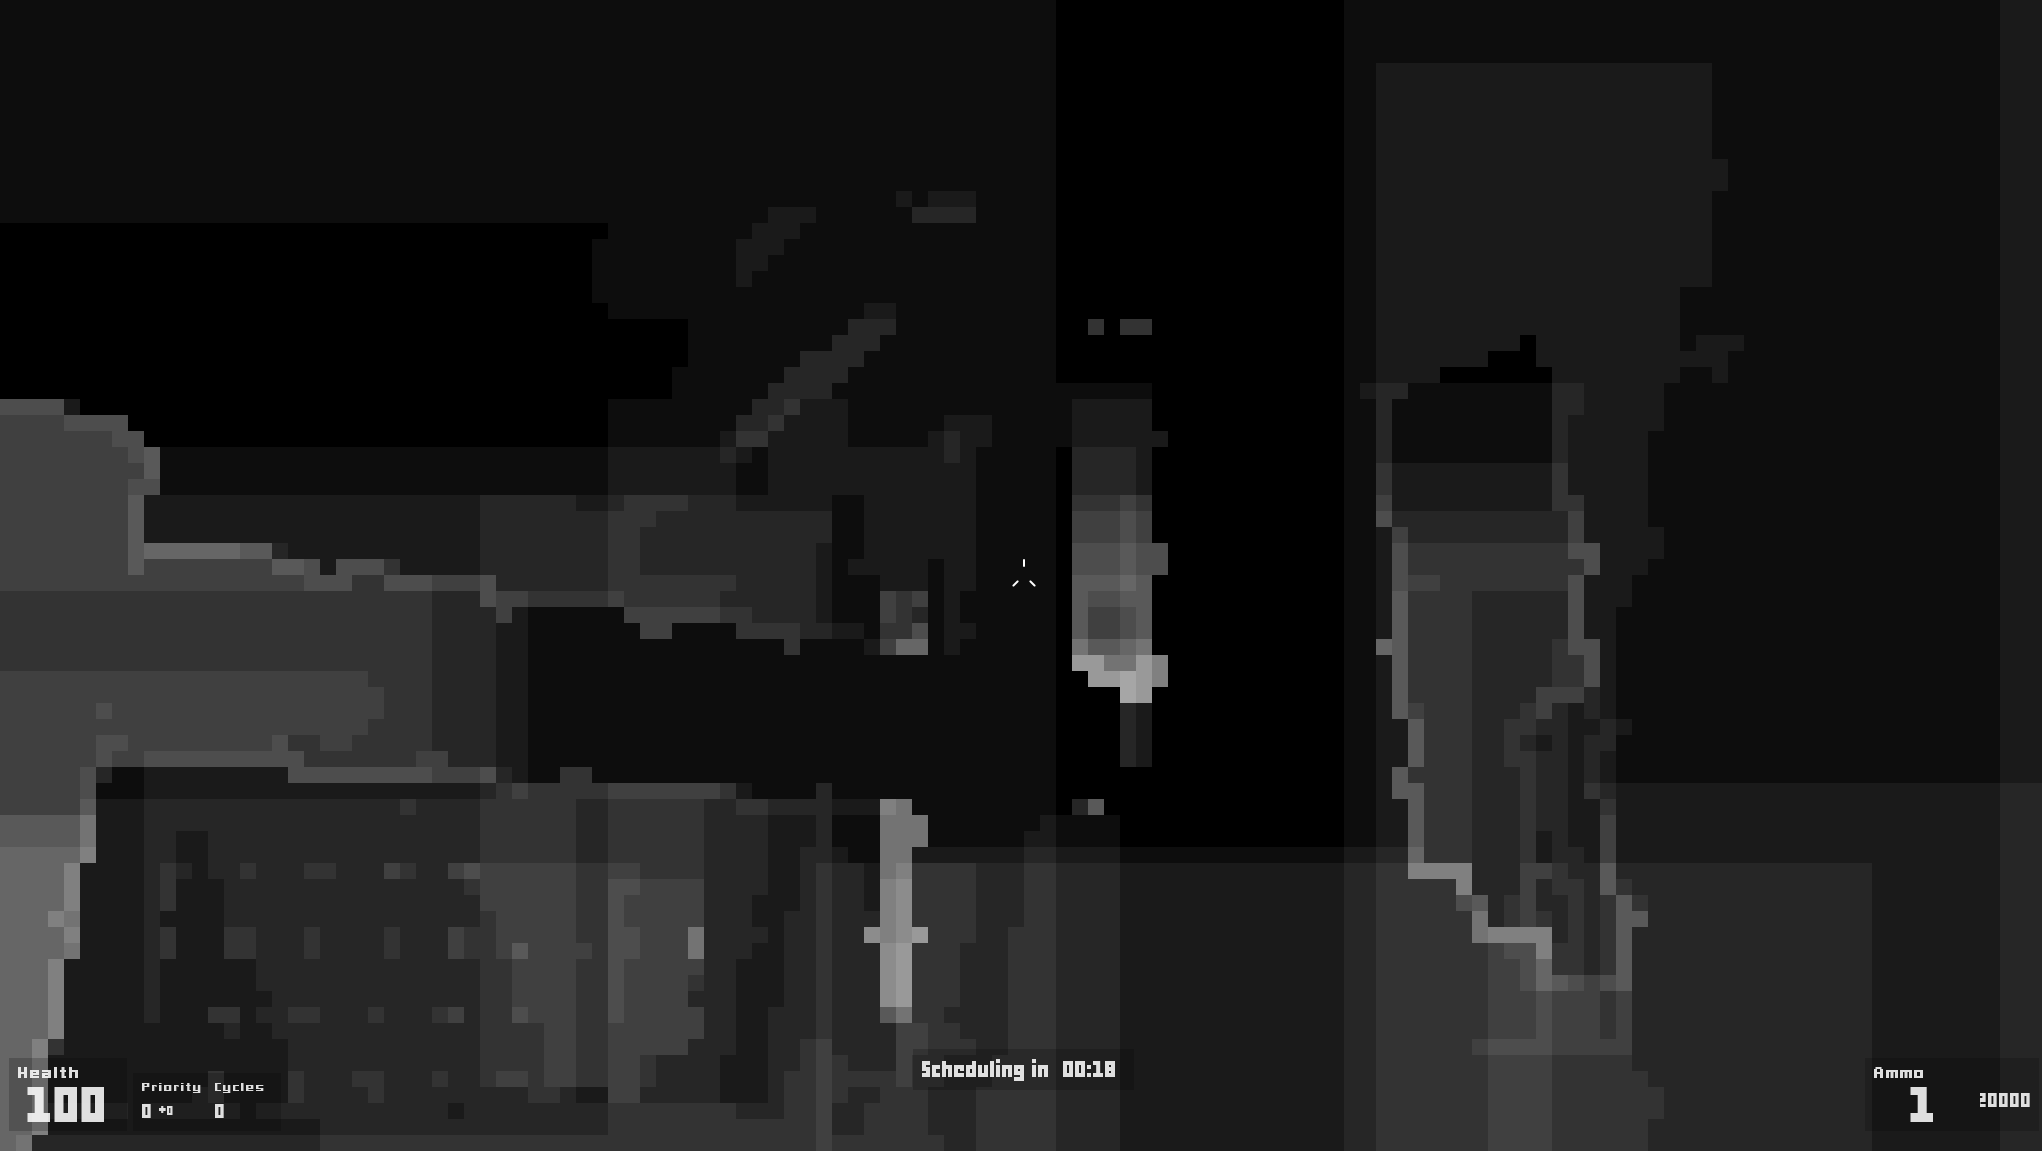
\includegraphics[width=1.0\textwidth]{img/tbds1.png}
  \end{minipage}
  \hspace{0.25cm}
  \begin{minipage}[b]{0.3\linewidth}
    \centering
    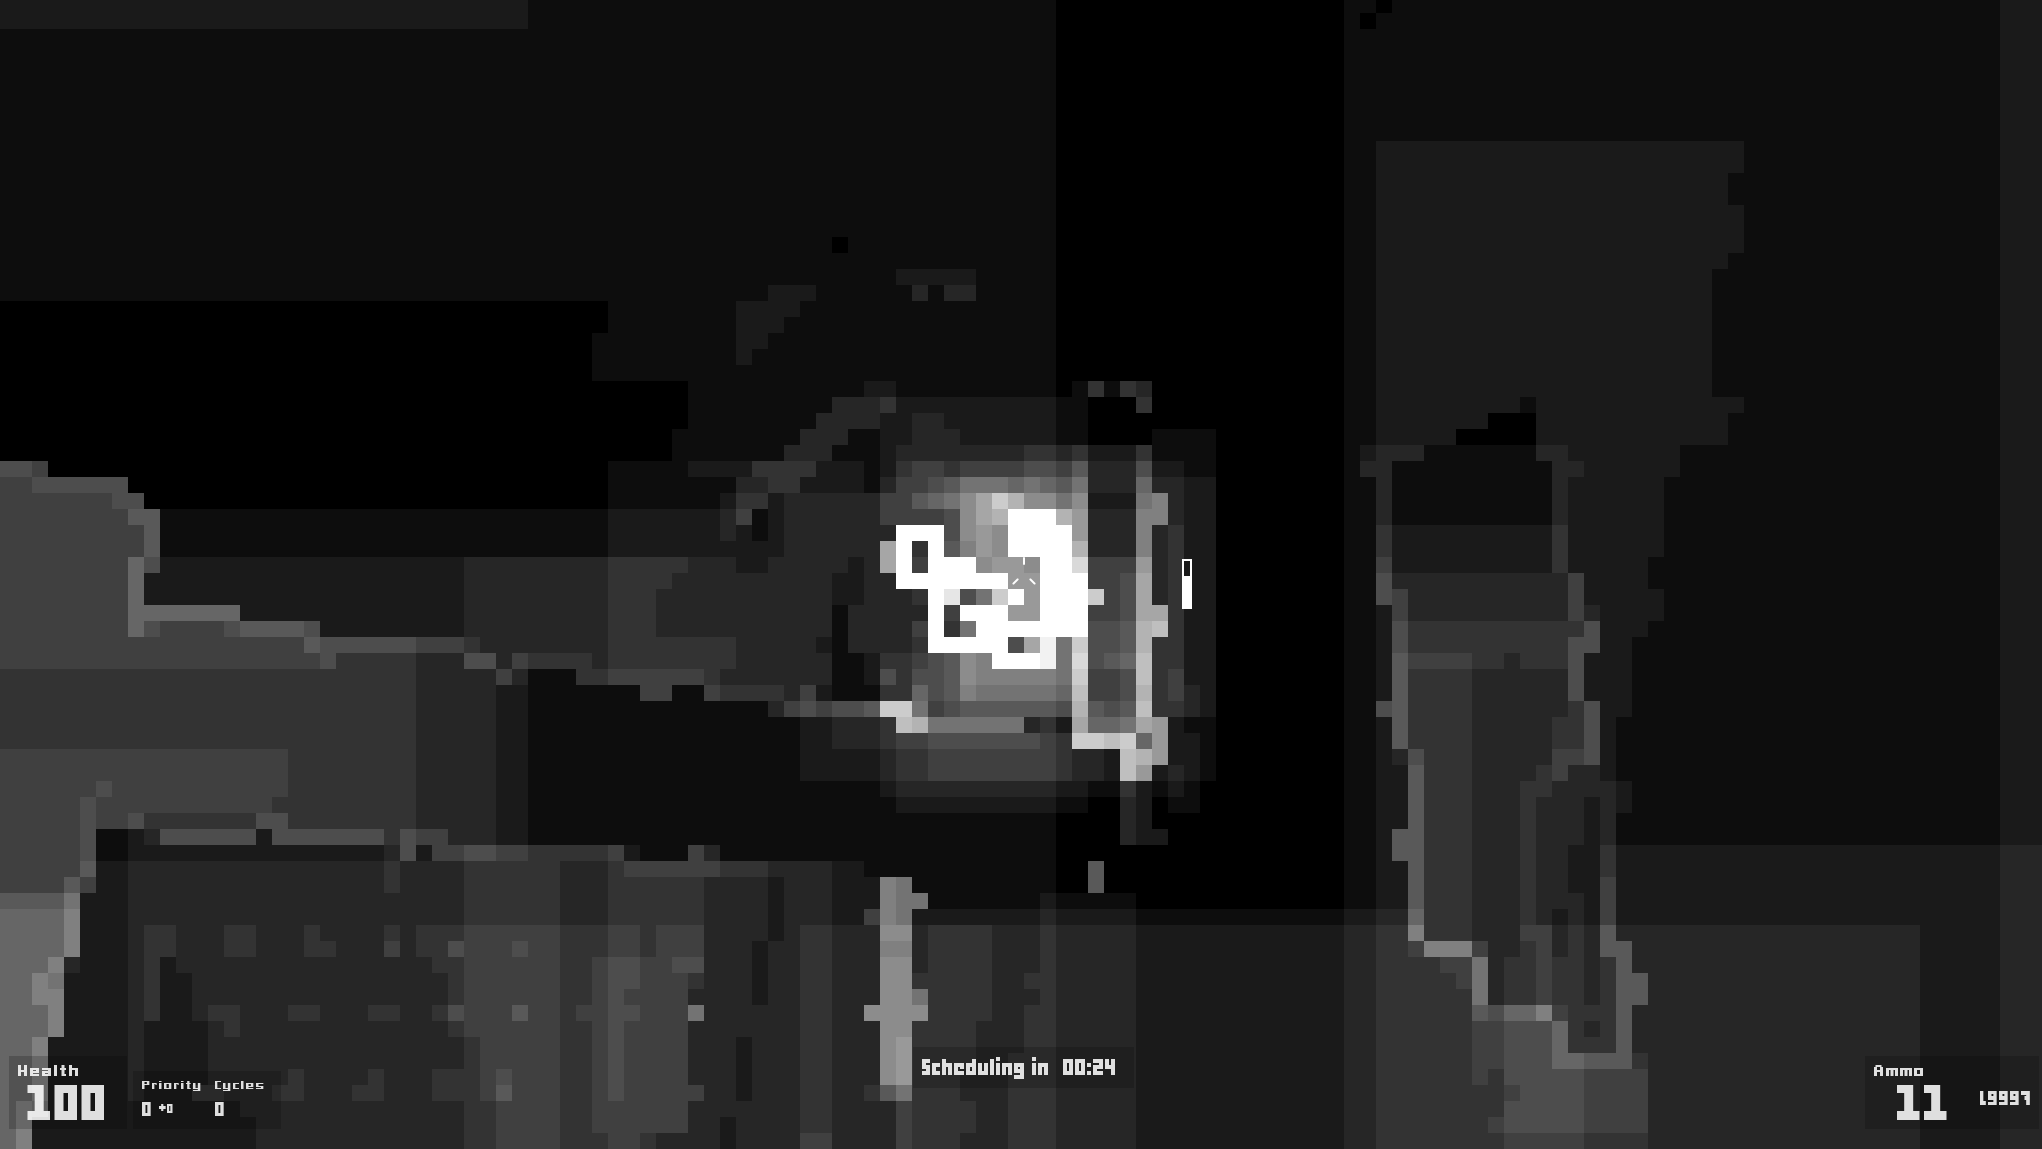
\includegraphics[width=1.0\textwidth]{img/tbds2.png}
  \end{minipage}
  \hspace{0.25cm}
  \begin{minipage}[b]{0.3\linewidth}
    \centering
    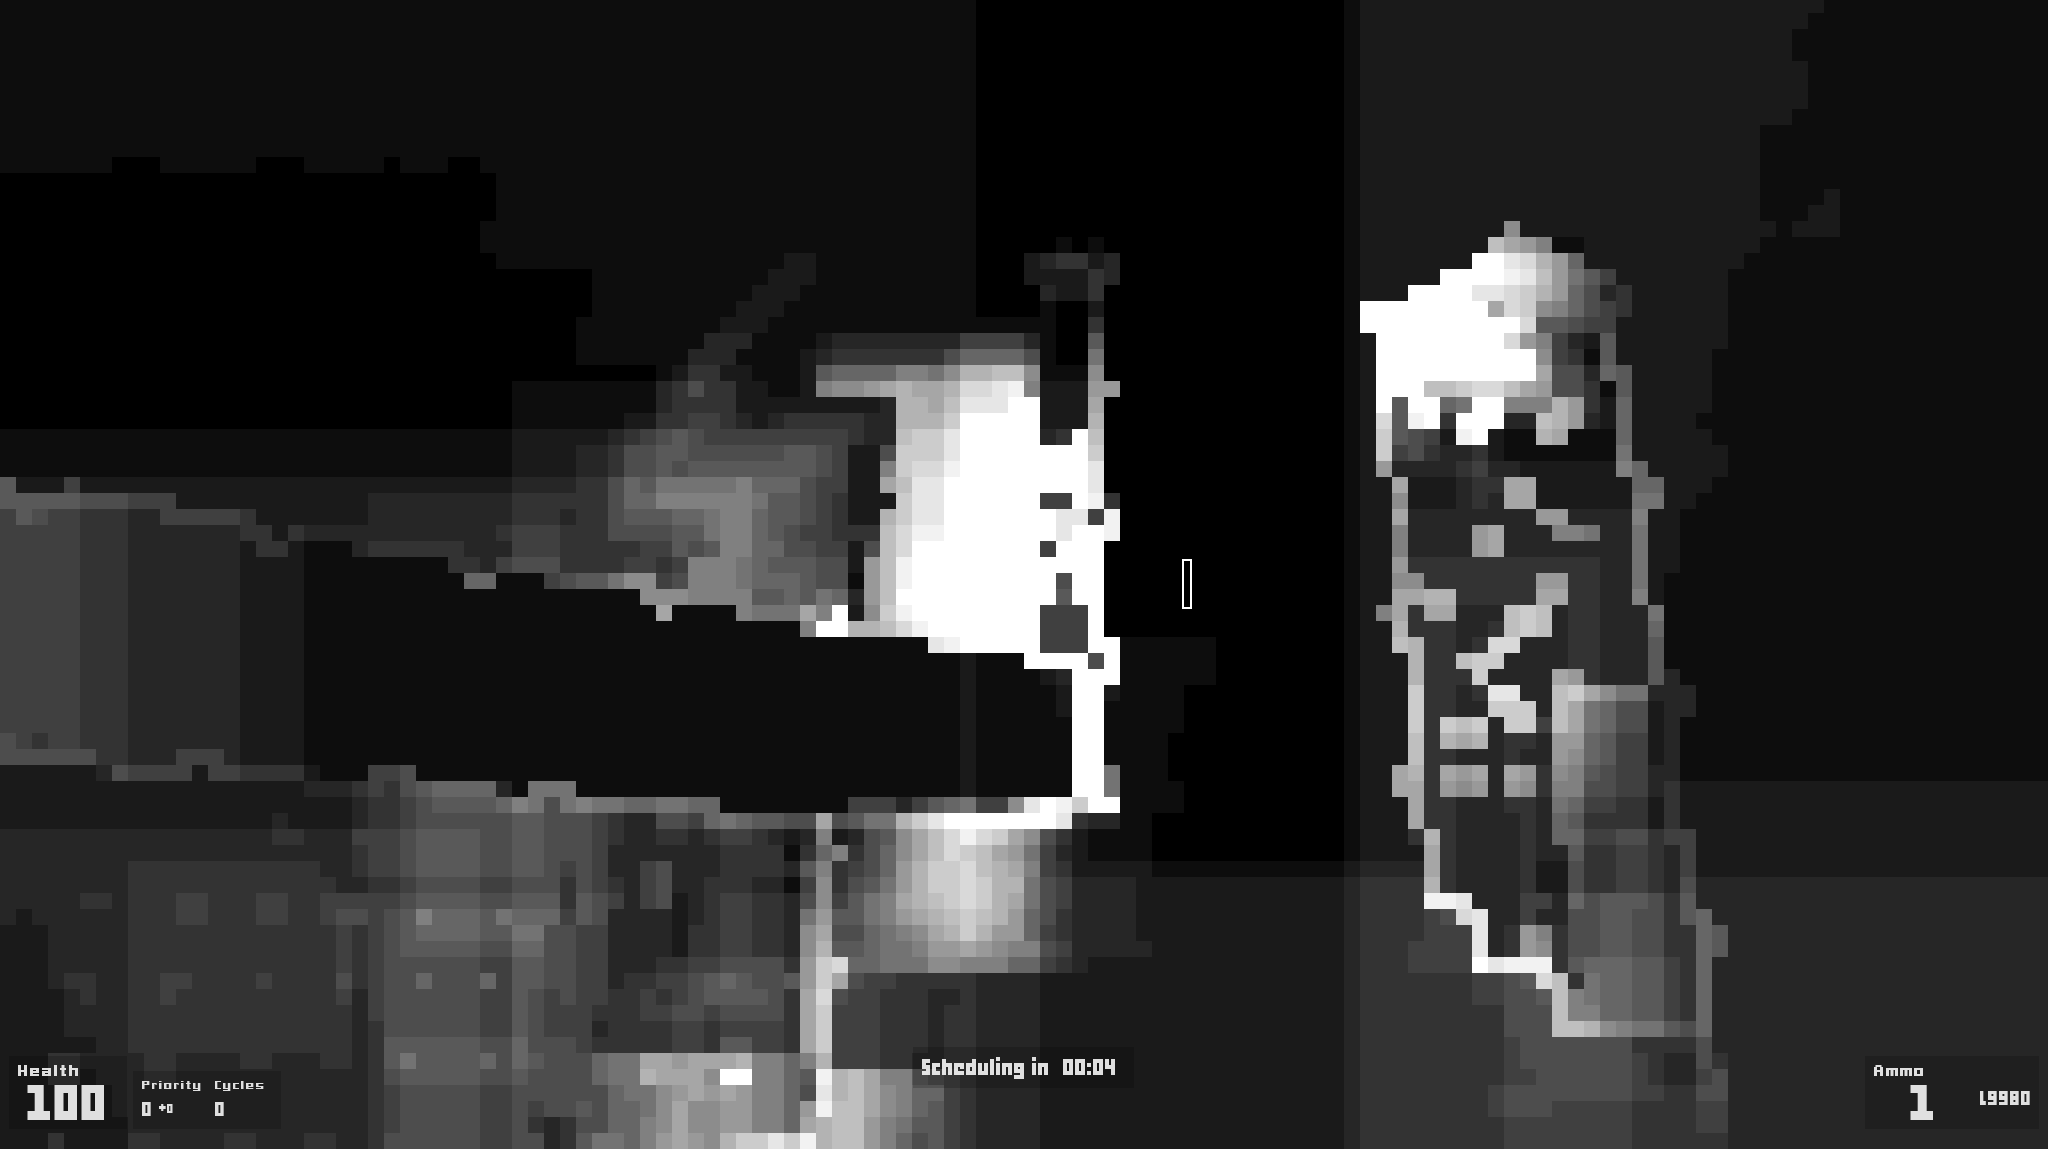
\includegraphics[width=1.0\textwidth]{img/tbds3.png}
  \end{minipage}
  \label{fig:tilingvisualization}
  \caption{\href{https://github.com/L0mion/xkill-source}{%
      Tile-based deferred shading using DirectCompute.}}
\end{figure}

\begin{figure}[ht]
  \begin{minipage}[b]{0.3\linewidth}
    \centering
    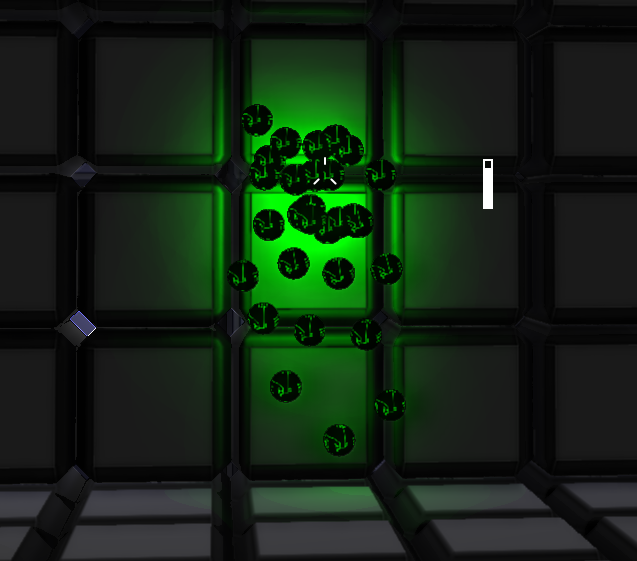
\includegraphics[width=1.0\textwidth]{img/tbds.png}
    \caption{AMD\textit{*≠}}
  \end{minipage}
  \hspace{0.25cm}
  \begin{minipage}[b]{0.3\linewidth}
    \centering
    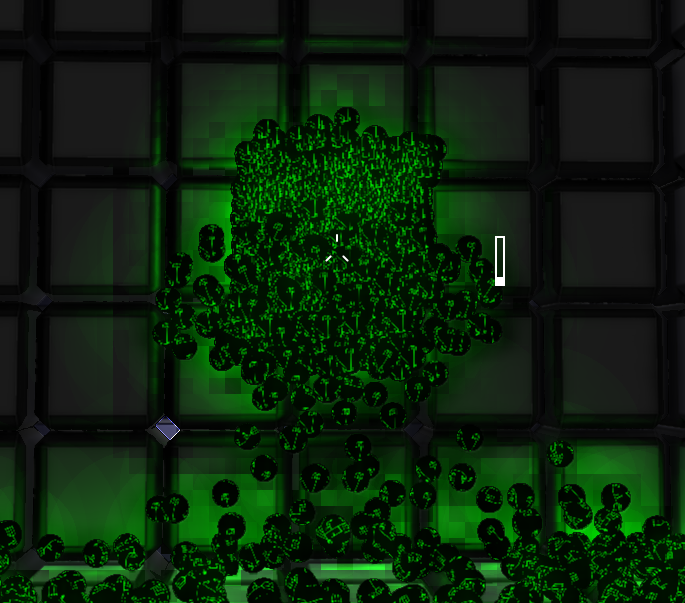
\includegraphics[width=1.0\textwidth]{img/tbds_error.png}
    \caption{NVIDIA\textit{*≠}}
  \end{minipage}
  \label{fig:tilingerror}
\end{figure}

\end{frame}

% REFERENCE DEVICE DRIVER
% The DirectX Reference Device Driver to the rescue!
\subsection{Reference Device Driver}
\begin{frame}
\frametitle{REFERENCE DEVICE DRIVER}

The Reference Device Driver or Reference Rasterizer:
\begin{itemize}
\item Shipped with the DirectX SDK
\item \textbf{Not} included in Windows run-times
\item Intended for debugging purposes:
  \begin{itemize}
  \item Feature testing
  \item Demonstration purposes
  \end{itemize}
\item Does feature some native instruction optimization, but all-in-all not intended for retail applications
\end{itemize}

\end{frame}

% GRAPHICS SIMULATION
\subsection{Graphics Simulation}
\begin{frame}
\frametitle{GRAPHICS SIMULATION}

\begin{itemize}
\item Common method of verifying GPU workloads, such as computer graphics, by eliminating dependency to third-party drivers and hardware
\item May also be practical for the purposes of extracting additional debugging or profiling data
\item Sometimes an unfortunate necessity on platforms lacking conformant hardware
  \begin{itemize}
  \item Pre-silicon
  \item Server systems
  \item Virtual platforms
  \end{itemize}
\item Often orders of magnitude too slow for complex applications
\end{itemize}

\end{frame}

% MICROSOFT WARP
\subsection{Microsoft WARP}
\begin{frame}
\frametitle{MICROSOFT WARP}

\href{http://msdn.microsoft.com/en-us/library/windows/desktop/gg615082(v=vs.85)%
  .aspx}{'...a high speed, fully conformant software rasterizer...':}
\begin{itemize}
\item Introduced in Direct3D 11
\item Derived from the Reference Device Driver
\item Included in Windows 7 and 8 runtimes
\end{itemize}

Optimized for CPU execution using:
\begin{itemize}
\item Thread pooling for modern multicore CPUs
\item Batch execution (possibly similar in concept to NVIDIA warps)
\item JIT compilation:
  \begin{itemize}
  \item x86 native instructions
  \item SSE2 and SSE4.1 SIMD
  \end{itemize}
\end{itemize}

See also: \href{http://www.mesa3d.org/llvmpipe.html}{the Gallium llvmpipe driver}

\end{frame}
